\documentclass[11pt,a4paper]{article}
\usepackage[margin=24mm,headheight=15pt]{geometry}
\usepackage[T1]{fontenc}
\usepackage{lmodern,microtype}
\usepackage{amsmath,amssymb,mathtools}
\usepackage{graphicx,tikz}
\usetikzlibrary{arrows.meta,positioning,calc,shapes.geometric}
\usepackage{booktabs,tabularx,array,enumitem}
\usepackage[section]{placeins}
\usepackage[font=small,labelfont=bf]{caption}
\captionsetup{hypcap=false}
\usepackage{xcolor,fancyhdr,titlesec}
\definecolor{ink}{HTML}{17324D}
\definecolor{teal}{HTML}{087F8C}
\definecolor{orange}{HTML}{BD622A}
\definecolor{muted}{HTML}{526575}
\colorlet{xc}{orange}\colorlet{zc}{teal}
\usepackage[colorlinks=true,linkcolor=teal,urlcolor=teal,citecolor=teal]{hyperref}
\hypersetup{pdftitle={Rotated Surface Codes},pdfauthor={}}
\newcommand{\ket}[1]{\lvert #1\rangle}
\newcommand{\bra}[1]{\langle #1\rvert}
\newcommand{\XL}{\overline{X}}
\newcommand{\ZL}{\overline{Z}}
\newcommand{\SL}{\mathcal{S}}
\newcommand{\cnot}{\operatorname{CNOT}}
\setlength{\parindent}{0pt}
\setlength{\parskip}{5pt}
\setlength{\emergencystretch}{2em}
\titleformat{\section}{\Large\bfseries\color{ink}}{\thesection}{0.6em}{}
\titleformat{\subsection}{\large\bfseries\color{ink}}{\thesubsection}{0.6em}{}
\pagestyle{fancy}\fancyhf{}
\fancyhead[L]{\small\color{muted} QUANTUM COMPUTING / FOUNDATIONS}
\fancyfoot[L]{\small\color{muted} Tutorial 03: Rotated Surface Codes}
\fancyfoot[R]{\small\thepage}
\renewcommand{\headrulewidth}{0.3pt}
\setlist[itemize]{nosep,leftmargin=1.5em}
\setlist[enumerate]{itemsep=3pt,leftmargin=1.5em}
\newcommand{\takeaway}[1]{\begin{quote}\color{ink}\textbf{#1}\end{quote}}
% Original editable TikZ figures. Coordinates and Pauli supports are checked by
% validate.py. X = orange; Z = teal throughout, including ZX spiders.
\tikzset{data/.style={circle,fill=ink,inner sep=1.6pt},
  zs/.style={circle,draw=zc,fill=zc!30,minimum size=6mm,inner sep=0pt},
  xs/.style={circle,draw=xc,fill=xc!30,minimum size=6mm,inner sep=0pt},
  wire/.style={thick,draw=ink},event/.style={circle,fill=ink,inner sep=2.2pt}}

% d odd; square data grid 0,...,d-1. Even bulk faces X, odd Z.
\newcommand{\rotpatch}[2]{%
\pgfmathtruncatemacro{\dm}{#1-1}
\pgfmathtruncatemacro{\df}{#1-2}
\foreach \x in {0,...,\df}{\foreach \y in {0,...,\df}{
 \pgfmathtruncatemacro{\parity}{mod(\x+\y,2)}
 \ifnum\parity=0 \def\col{xc}\def\typ{X}\else\def\col{zc}\def\typ{Z}\fi
 \filldraw[fill=\col!15,draw=\col!45] (\x,\y) rectangle +(1,1);
 \node[text=\col,font=\scriptsize] at (\x+.5,\y+.5) {$\typ$};
}}
\foreach \i in {0,...,\df}{
 \pgfmathtruncatemacro{\parity}{mod(\i,2)}
 \ifnum\parity=0
  \filldraw[fill=zc!15,draw=zc!45] (\i,0)--(\i+.5,-.45)--(\i+1,0)--cycle;
  \node[text=zc,font=\tiny] at (\i+.5,-.17) {$Z$};
  \filldraw[fill=xc!15,draw=xc!45] (\dm,\i)--(\dm+.45,\i+.5)--(\dm,\i+1)--cycle;
  \node[text=xc,font=\tiny] at (\dm+.17,\i+.5) {$X$};
 \else
  \filldraw[fill=zc!15,draw=zc!45] (\i,\dm)--(\i+.5,\dm+.45)--(\i+1,\dm)--cycle;
  \node[text=zc,font=\tiny] at (\i+.5,\dm+.17) {$Z$};
  \filldraw[fill=xc!15,draw=xc!45] (0,\i)--(-.45,\i+.5)--(0,\i+1)--cycle;
  \node[text=xc,font=\tiny] at (-.17,\i+.5) {$X$};
 \fi
}
\foreach \x in {0,...,\dm}{\foreach \y in {0,...,\dm}{
 \node[data] at (\x,\y) {};
 \ifnum#2=1
  \pgfmathtruncatemacro{\qid}{#1*\y+\x}
  \node[font=\tiny,anchor=south west,fill=white,inner sep=.3pt] at (\x+.035,\y+.035) {\qid};
 \fi
}}
}

\newcommand{\layoutcomparison}{%
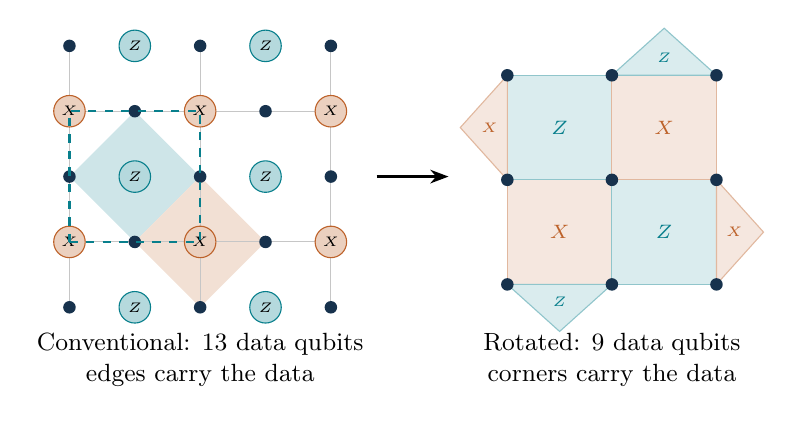
\begin{tikzpicture}[scale=.83]
\begin{scope}
\fill[zc!20] (0,2)--(1,1)--(2,2)--(1,3)--cycle;
\fill[xc!20] (2,0)--(1,1)--(2,2)--(3,1)--cycle;
\foreach \x in {0,2,4}{\draw[gray!45] (\x,0)--(\x,4);}
\foreach \y in {1,3}{\draw[gray!45] (0,\y)--(4,\y);}
\foreach \x in {0,...,4}{\foreach \y in {0,...,4}{
 \pgfmathtruncatemacro{\p}{mod(\x+\y,2)}
 \ifnum\p=0 \node[data] at (\x,\y) {};
 \else
  \pgfmathtruncatemacro{\q}{mod(\x,2)}
  \ifnum\q=0 \node[xs,minimum size=4mm,font=\tiny] at (\x,\y) {$X$};
  \else \node[zs,minimum size=4mm,font=\tiny] at (\x,\y) {$Z$};\fi
 \fi
}}
\draw[zc,thick,dashed] (0,1)--(2,1)--(2,3)--(0,3)--cycle;
\node[font=\small,align=center] at (2,-.8) {Conventional: 13 data qubits\\edges carry the data};
\end{scope}
\draw[-{Stealth},thick] (4.7,2)--(5.8,2);
\begin{scope}[shift={(6.7,.35)},scale=1.6]
\rotpatch{3}{0}
\end{scope}
\node[font=\small,align=center] at (8.3,-.8) {Rotated: 9 data qubits\\corners carry the data};
\end{tikzpicture}}

\newcommand{\detailedpatch}{%
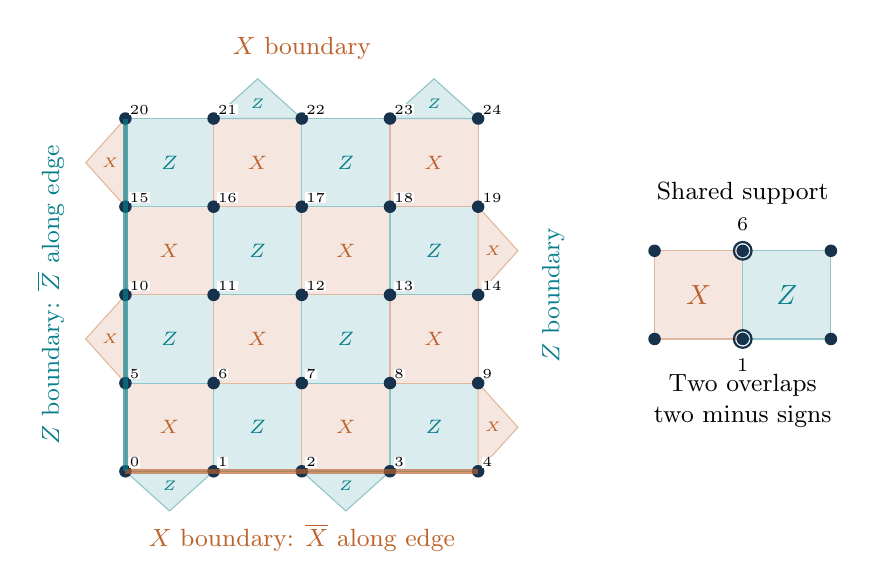
\begin{tikzpicture}[scale=1.12]
\rotpatch{5}{1}
\draw[xc,line width=2pt,opacity=.65] (0,0)--(4,0);
\draw[zc,line width=2pt,opacity=.65] (0,0)--(0,4);
\node[text=xc,font=\small] at (2,4.8) {$X$ boundary};
\node[text=xc,font=\small] at (2,-.75) {$X$ boundary: $\XL$ along edge};
\node[text=zc,rotate=90,font=\small] at (-.85,2) {$Z$ boundary: $\ZL$ along edge};
\node[text=zc,rotate=90,font=\small] at (4.85,2) {$Z$ boundary};
\begin{scope}[shift={(6,1.5)}]
\filldraw[fill=xc!15,draw=xc!45] (0,0) rectangle (1,1);
\filldraw[fill=zc!15,draw=zc!45] (1,0) rectangle (2,1);
\node[text=xc] at (.5,.5) {$X$};\node[text=zc] at (1.5,.5) {$Z$};
\foreach \x in {0,1,2}{\foreach \y in {0,1}{\node[data] at (\x,\y) {};}}
\draw[ink,thick] (1,0) circle (.1) (1,1) circle (.1);
\node[font=\scriptsize,anchor=north] at (1,-.12) {1};
\node[font=\scriptsize,anchor=south] at (1,1.12) {6};
\node[font=\small] at (1,1.65) {Shared support};
\node[font=\small,align=center] at (1,-.7) {Two overlaps\\two minus signs};
\end{scope}
\end{tikzpicture}}

\newcommand{\schedules}{%
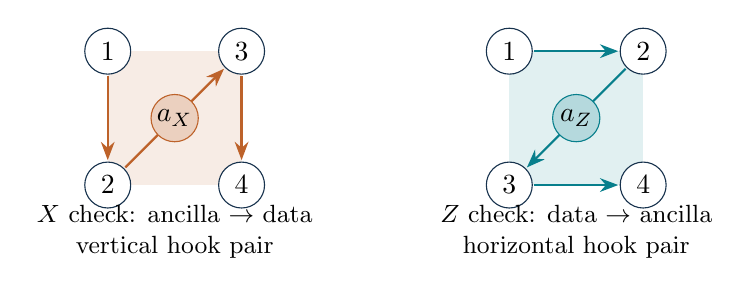
\begin{tikzpicture}[scale=.85]
\begin{scope}
\fill[xc!12] (0,0) rectangle (2,2);
\draw[xc,thick,-{Stealth},shorten <=9pt,shorten >=9pt] (0,2)--(0,0);
\draw[xc,thick,-{Stealth},shorten <=9pt,shorten >=9pt] (0,0)--(2,2);
\draw[xc,thick,-{Stealth},shorten <=9pt,shorten >=9pt] (2,2)--(2,0);
\node[xs] at (1,1) {$a_X$};
\foreach \x/\y/\n in {0/2/1,0/0/2,2/2/3,2/0/4}{\node[circle,fill=white,draw=ink,inner sep=3pt] at (\x,\y) {\n};}
\node[font=\small,align=center] at (1,-.7) {$X$ check: ancilla $\to$ data\\vertical hook pair};
\end{scope}
\begin{scope}[xshift=6cm]
\fill[zc!12] (0,0) rectangle (2,2);
\draw[zc,thick,-{Stealth},shorten <=9pt,shorten >=9pt] (0,2)--(2,2);
\draw[zc,thick,-{Stealth},shorten <=9pt,shorten >=9pt] (2,2)--(0,0);
\draw[zc,thick,-{Stealth},shorten <=9pt,shorten >=9pt] (0,0)--(2,0);
\node[zs] at (1,1) {$a_Z$};
\foreach \x/\y/\n in {0/2/1,2/2/2,0/0/3,2/0/4}{\node[circle,fill=white,draw=ink,inner sep=3pt] at (\x,\y) {\n};}
\node[font=\small,align=center] at (1,-.7) {$Z$ check: data $\to$ ancilla\\horizontal hook pair};
\end{scope}
\end{tikzpicture}}

\newcommand{\errorpatch}{%
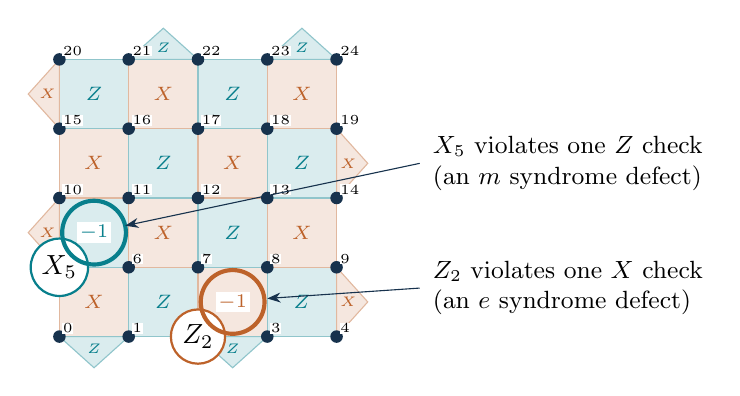
\begin{tikzpicture}[scale=.88]
\rotpatch{5}{1}
\node[circle,fill=white,draw=zc,thick,inner sep=2pt] at (0,1) {$X_5$};
\node[circle,fill=white,draw=xc,thick,inner sep=2pt] at (2,0) {$Z_2$};
\draw[zc,line width=1.5pt] (.5,1.5) circle (.46);
\node[fill=white,inner sep=1pt,text=zc,font=\scriptsize] at (.5,1.5) {$-1$};
\draw[xc,line width=1.5pt] (2.5,.5) circle (.46);
\node[fill=white,inner sep=1pt,text=xc,font=\scriptsize] at (2.5,.5) {$-1$};
\draw[-{Stealth},ink] (5.2,2.5)--(.95,1.6);
\node[anchor=west,font=\small,align=left] at (5.25,2.5)
  {$X_5$ violates one $Z$ check\\(an $m$ syndrome defect)};
\draw[-{Stealth},ink] (5.2,.7)--(3,.55);
\node[anchor=west,font=\small,align=left] at (5.25,.7)
  {$Z_2$ violates one $X$ check\\(an $e$ syndrome defect)};
\end{tikzpicture}}

% Abstract square: horizontal X edges, vertical Z edges.
\newcommand{\squarepatch}[1][1]{%
\fill[ink!3] (0,0) rectangle (2,2);
\draw[xc,line width=2pt] (0,0)--(2,0) (0,2)--(2,2);
\draw[zc,line width=2pt] (0,0)--(0,2) (2,0)--(2,2);
\ifnum#1=1
\node[text=xc,font=\scriptsize] at (1,2.2) {$X$};
\node[text=xc,font=\scriptsize] at (1,-.2) {$X$};
\node[text=zc,font=\scriptsize] at (-.2,1) {$Z$};
\node[text=zc,font=\scriptsize] at (2.2,1) {$Z$};\fi}

\newcommand{\abstractstrings}{%
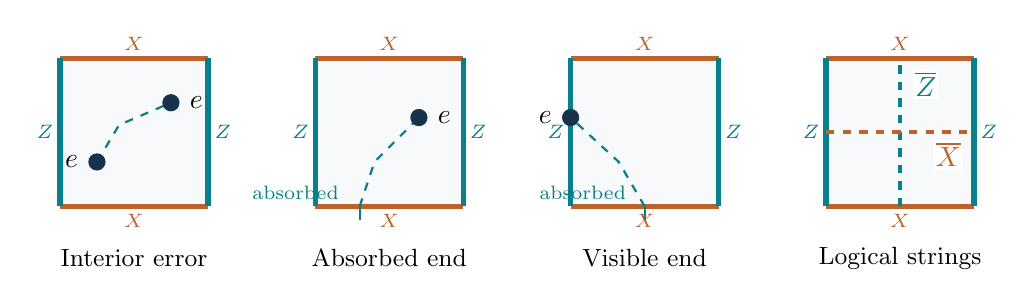
\begin{tikzpicture}[scale=.94]
\squarepatch
\draw[zc,thick,dashed] (.5,.6)--(.8,1.1)--(1.5,1.4);
\node[event,label=left:$e$] at (.5,.6) {};
\node[event,label=right:$e$] at (1.5,1.4) {};
\node[font=\small,align=center] at (1,-.7) {Interior error};
\begin{scope}[xshift=3.45cm]
\squarepatch
\draw[zc,thick,dashed] (.6,0)--(.8,.6)--(1.4,1.2);
\draw[zc,thick] (.6,0)--(.6,-.18);
\node[text=zc,font=\scriptsize,anchor=east] at (.45,.18) {absorbed};
\node[event,label=right:$e$] at (1.4,1.2) {};
\node[font=\small,align=center] at (1,-.7) {Absorbed end};
\end{scope}
\begin{scope}[xshift=6.9cm]
\squarepatch
\draw[zc,thick,dashed] (1,0)--(.65,.6)--(0,1.2);
\draw[zc,thick] (1,0)--(1,-.18);
\node[text=zc,font=\scriptsize,anchor=east] at (.88,.18) {absorbed};
\node[event,label=left:$e$] at (0,1.2) {};
\node[font=\small,align=center] at (1,-.7) {Visible end};
\end{scope}
\begin{scope}[xshift=10.35cm]
\squarepatch
\draw[zc,line width=1.5pt,dashed] (1,0)--(1,2);
\draw[xc,line width=1.5pt,dashed] (0,1)--(2,1);
\node[fill=white,inner sep=1pt,text=zc] at (1.35,1.65) {$\ZL$};
\node[fill=white,inner sep=1pt,text=xc] at (1.65,.7) {$\XL$};
\node[font=\small,align=center] at (1,-.7) {Logical strings};
\end{scope}
\end{tikzpicture}}

\newcommand{\memorydiagram}{%
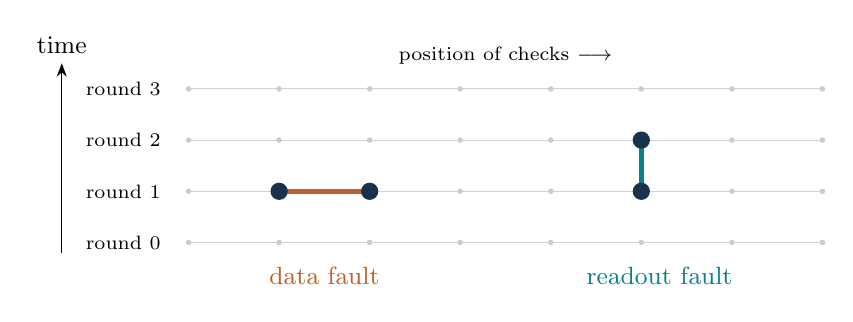
\begin{tikzpicture}[x=1.15cm,y=.65cm]
\foreach \t in {0,1,2,3}{
 \draw[gray!35] (0,\t)--(7,\t);
 \node[anchor=east,font=\scriptsize] at (-.2,\t) {round $\t$};
 \foreach \x in {0,...,7}{\fill[gray!40] (\x,\t) circle (1pt);}
}
\draw[-{Stealth}] (-1.4,-.2)--(-1.4,3.5) node[above,font=\small] {time};
\draw[xc,line width=2pt] (1,1)--(2,1);
\node[event] at (1,1) {};\node[event] at (2,1) {};
\draw[zc,line width=2pt] (5,1)--(5,2);
\node[event] at (5,1) {};\node[event] at (5,2) {};
\node[font=\small,text=xc] at (1.5,-.65) {data fault};
\node[font=\small,text=zc] at (5.2,-.65) {readout fault};
\node[font=\scriptsize] at (3.5,3.65) {position of checks $\longrightarrow$};
\end{tikzpicture}}

\newcommand{\surgerypair}[1]{%
\begin{scope}[scale=.7]
\squarepatch[0]
\begin{scope}[xshift=2.5cm]\squarepatch[0]\end{scope}
\node at (1,1) {$1$};\node at (3.5,1) {$2$};
\ifnum#1=1
\fill[zc!25] (2,-.02) rectangle (2.5,2.02);
\draw[zc,thick] (2,0)--(2.5,0) (2,2)--(2.5,2);
\fi
\end{scope}}
\newcommand{\surgerydiagram}{%
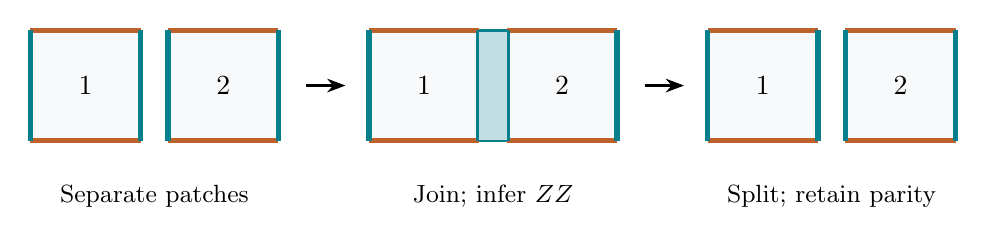
\begin{tikzpicture}
\surgerypair{0}
\node[font=\small] at (1.575,-.7) {Separate patches};
\draw[-{Stealth},thick] (3.5,.7)--(4,.7);
\begin{scope}[xshift=4.3cm]\surgerypair{1}\end{scope}
\node[font=\small] at (5.875,-.7) {Join; infer $ZZ$};
\draw[-{Stealth},thick] (7.8,.7)--(8.3,.7);
\begin{scope}[xshift=8.6cm]\surgerypair{0}\end{scope}
\node[font=\small] at (10.175,-.7) {Split; retain parity};
\end{tikzpicture}}

\newcommand{\cnotstage}[1]{%
\begin{scope}[scale=.55]
\squarepatch[0]\node at (1,1) {$C$};
\begin{scope}[xshift=2.6cm]\squarepatch[0]\node at (1,1) {$A$};\end{scope}
\begin{scope}[shift={(2.6,-2.6)}]\squarepatch[0]\node at (1,1) {$T$};\end{scope}
\ifnum#1=1 \fill[zc!40] (2,0) rectangle (2.6,2);\fi
\ifnum#1=2 \fill[xc!40] (2.6,-.6) rectangle (4.6,0);\fi
\ifnum#1=3 \node[fill=white,font=\small] at (3.6,1) {$Z_A$};\fi
\end{scope}}
\newcommand{\cnotpatches}{%
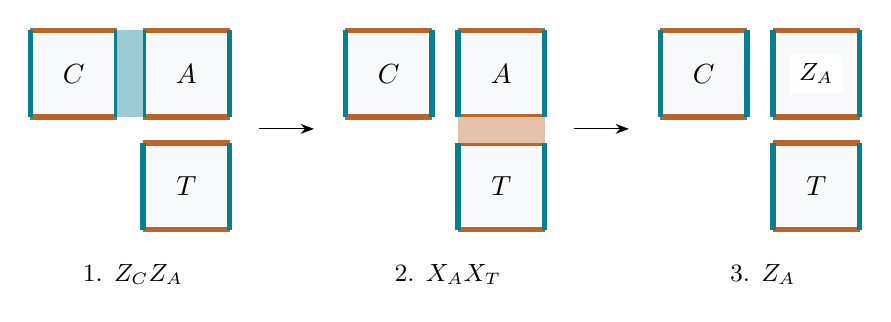
\begin{tikzpicture}
\cnotstage{1}\node[font=\small] at (1.3,-2) {1. $Z_CZ_A$};
\draw[-{Stealth}] (2.9,-.15)--(3.6,-.15);
\begin{scope}[xshift=4cm]\cnotstage{2}\end{scope}
\node[font=\small] at (5.3,-2) {2. $X_AX_T$};
\draw[-{Stealth}] (6.9,-.15)--(7.6,-.15);
\begin{scope}[xshift=8cm]\cnotstage{3}\end{scope}
\node[font=\small] at (9.3,-2) {3. $Z_A$};
\end{tikzpicture}}

\newcommand{\zxdiagram}{%
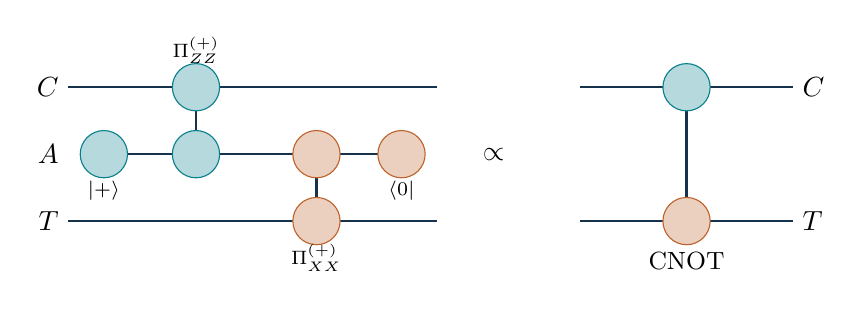
\begin{tikzpicture}[x=.9cm,y=.85cm]
\node[anchor=east] at (0,2) {$C$};
\node[anchor=east] at (0,1) {$A$};
\node[anchor=east] at (0,0) {$T$};
\draw[wire] (0,2)--(5.2,2) (0,0)--(5.2,0) (.5,1)--(4.7,1);
\draw[wire] (1.8,2)--(1.8,1) (3.5,1)--(3.5,0);
\node[zs] at (1.8,2) {};\node[zs] at (1.8,1) {};
\node[xs] at (3.5,1) {};\node[xs] at (3.5,0) {};
\node[zs] at (.5,1) {};\node[xs] at (4.7,1) {};
\node[font=\scriptsize] at (.5,.45) {$\ket{+}$};
\node[font=\scriptsize] at (4.7,.45) {$\bra{0}$};
\node[font=\scriptsize] at (1.8,2.55) {$\Pi_{ZZ}^{(+)}$};
\node[font=\scriptsize] at (3.5,-.55) {$\Pi_{XX}^{(+)}$};
\node at (6,1) {$\propto$};
\begin{scope}[xshift=6.5cm]
\draw[wire] (0,2)--(3,2) (0,0)--(3,0) (1.5,0)--(1.5,2);
\node[zs] at (1.5,2) {};\node[xs] at (1.5,0) {};
\node[font=\small] at (1.5,-.6) {CNOT};
\node[anchor=west] at (3,2) {$C$};\node[anchor=west] at (3,0) {$T$};
\end{scope}
\end{tikzpicture}}

% A concrete circuit for the lower-left X check: data order 5,0,6,1.
\newcommand{\hookcircuit}{%
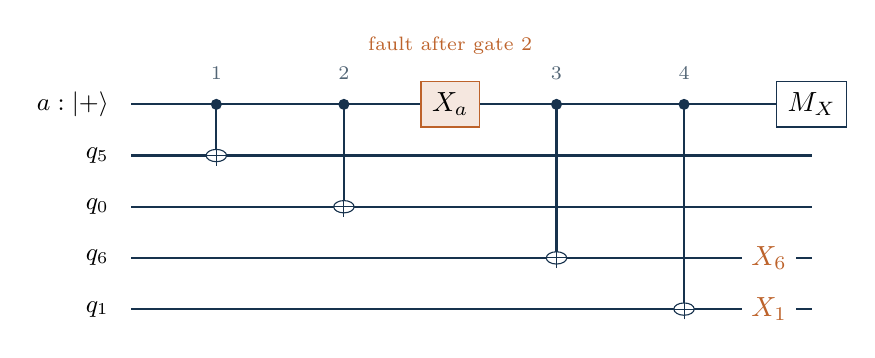
\begin{tikzpicture}[x=1.08cm,y=.65cm]
\foreach \y/\label in {4/{a:\ket+},3/{q_5},2/{q_0},1/{q_6},0/{q_1}}{
 \draw[wire] (0,\y)--(8,\y);
 \node[anchor=east,font=\small] at (-.15,\y) {$\label$};
}
\foreach \x/\y/\n in {1/3/1,2.5/2/2,5/1/3,6.5/0/4}{
 \draw[wire] (\x,4)--(\x,\y);
 \fill[ink] (\x,4) circle (2pt);
 \draw[ink,fill=white] (\x,\y) circle (.12);
 \draw[ink] (\x-.12,\y)--(\x+.12,\y) (\x,\y-.2)--(\x,\y+.2);
 \node[font=\scriptsize,text=muted] at (\x,4.6) {\n};
}
\node[draw=xc,fill=xc!15,inner sep=4pt] at (3.75,4) {$X_a$};
\node[text=xc,font=\scriptsize] at (3.75,5.15) {fault after gate 2};
\node[draw=ink,fill=white,inner sep=4pt] at (8,4) {$M_X$};
\node[fill=white,text=xc] at (7.5,1) {$X_6$};
\node[fill=white,text=xc] at (7.5,0) {$X_1$};
\end{tikzpicture}}

\newcommand{\pathdeformation}{%
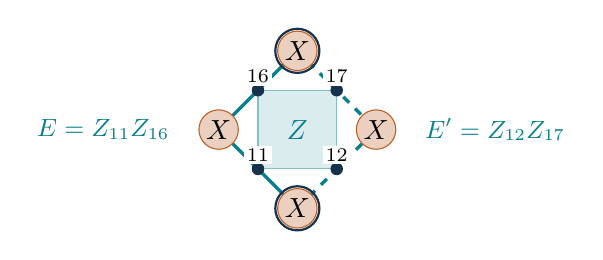
\begin{tikzpicture}[scale=1.0]
\filldraw[fill=zc!15,draw=zc!50] (0,0) rectangle (1,1);
\node[text=zc] at (.5,.5) {$Z$};
\draw[zc,very thick] (.5,-.5)--(-.5,.5)--(.5,1.5);
\draw[zc,very thick,dashed] (.5,-.5)--(1.5,.5)--(.5,1.5);
\foreach \x/\y in {-.5/.5,.5/-.5,1.5/.5,.5/1.5}{
 \node[xs,minimum size=5mm] at (\x,\y) {$X$};}

\foreach \x/\y/\q in {0/0/11,1/0/12,0/1/16,1/1/17}{
 \node[data] at (\x,\y) {};
 \node[fill=white,inner sep=1pt,font=\scriptsize,anchor=south] at (\x,\y+.05) {\q};}
\node[font=\small,anchor=east,text=zc] at (-1,.5) {$E=Z_{11}Z_{16}$};
\node[font=\small,anchor=west,text=zc] at (2,.5) {$E'=Z_{12}Z_{17}$};
\draw[ink,thick] (.5,-.5) circle (.28) (.5,1.5) circle (.28);
\end{tikzpicture}}

% Rectangular merged patch, data x=0..6,y=0..2; bridge x=3.
\newcommand{\physicalseam}{%
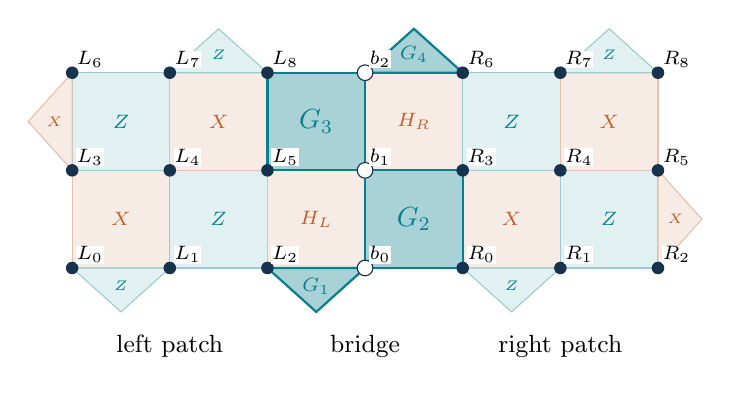
\begin{tikzpicture}[scale=1.24]
\foreach \x in {0,...,5}{\foreach \y in {0,1}{
 \pgfmathtruncatemacro{\p}{mod(\x+\y,2)}
 \ifnum\p=0 \def\cc{xc}\def\tt{X}\else \def\cc{zc}\def\tt{Z}\fi
 \filldraw[fill=\cc!12,draw=\cc!40] (\x,\y) rectangle +(1,1);
 \node[text=\cc,font=\scriptsize] at (\x+.5,\y+.5) {$\tt$};
}}
\foreach \x in {0,2,4}{
 \filldraw[fill=zc!12,draw=zc!40] (\x,0)--(\x+.5,-.45)--(\x+1,0)--cycle;
 \node[text=zc,font=\tiny] at (\x+.5,-.18) {$Z$};
}
\foreach \x in {1,3,5}{
 \filldraw[fill=zc!12,draw=zc!40] (\x,2)--(\x+.5,2.45)--(\x+1,2)--cycle;
 \node[text=zc,font=\tiny] at (\x+.5,2.18) {$Z$};
}
\filldraw[fill=xc!12,draw=xc!40] (0,1)--(-.45,1.5)--(0,2)--cycle;
\node[text=xc,font=\tiny] at (-.18,1.5) {$X$};
\filldraw[fill=xc!12,draw=xc!40] (6,0)--(6.45,.5)--(6,1)--cycle;
\node[text=xc,font=\tiny] at (6.18,.5) {$X$};
\filldraw[fill=zc!35,draw=zc,thick] (2,0)--(2.5,-.45)--(3,0)--cycle;
\filldraw[fill=zc!35,draw=zc,thick] (3,0) rectangle (4,1);
\filldraw[fill=zc!35,draw=zc,thick] (2,1) rectangle (3,2);
\filldraw[fill=zc!35,draw=zc,thick] (3,2)--(3.5,2.45)--(4,2)--cycle;
\node[text=zc,font=\scriptsize] at (2.5,-.19) {$G_1$};
\node[text=zc] at (3.5,.5) {$G_2$};
\node[text=zc] at (2.5,1.5) {$G_3$};
\node[text=zc,font=\scriptsize] at (3.5,2.19) {$G_4$};
\node[fill=xc!12,text=xc,font=\scriptsize] at (2.5,.5) {$H_L$};
\node[fill=xc!12,text=xc,font=\scriptsize] at (3.5,1.5) {$H_R$};
\foreach \x in {0,...,6}{\foreach \y in {0,1,2}{
 \ifnum\x<3
  \pgfmathtruncatemacro{\j}{3*\y+\x}\def\lab{L_{\j}}
  \node[data] at (\x,\y) {};
 \else\ifnum\x=3
  \def\lab{b_{\y}}\node[circle,draw=ink,fill=white,inner sep=2pt] at (\x,\y) {};
 \else
  \pgfmathtruncatemacro{\j}{3*\y+\x-4}\def\lab{R_{\j}}
  \node[data] at (\x,\y) {};
 \fi\fi
 \node[font=\scriptsize,anchor=south west,fill=white,inner sep=.3pt] at (\x+.035,\y+.04) {$\lab$};
}}
\node[font=\small] at (1,-.8) {left patch};
\node[font=\small] at (3,-.8) {bridge};
\node[font=\small] at (5,-.8) {right patch};
\end{tikzpicture}}

\newcommand{\spiderbasics}{%
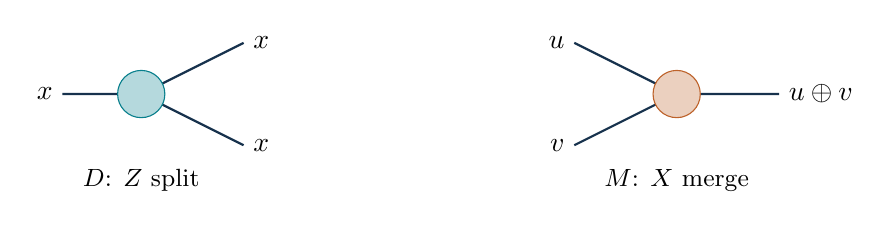
\begin{tikzpicture}[x=1cm,y=1cm]
\draw[wire] (0,0)--(1,0)--(2.3,.65) (1,0)--(2.3,-.65);
\node[zs] at (1,0) {};
\node[anchor=east] at (0,0) {$x$};
\node[anchor=west] at (2.3,.65) {$x$};\node[anchor=west] at (2.3,-.65) {$x$};
\node[font=\small] at (1,-1.1) {$D$: $Z$ split};
\begin{scope}[xshift=6.5cm]
\draw[wire] (0,.65)--(1.3,0)--(2.6,0) (0,-.65)--(1.3,0);
\node[xs] at (1.3,0) {};
\node[anchor=east] at (0,.65) {$u$};\node[anchor=east] at (0,-.65) {$v$};
\node[anchor=west] at (2.6,0) {$u\oplus v$};
\node[font=\small] at (1.3,-1.1) {$M$: $X$ merge};
\end{scope}
\end{tikzpicture}}

\renewcommand{\zxdiagram}{%
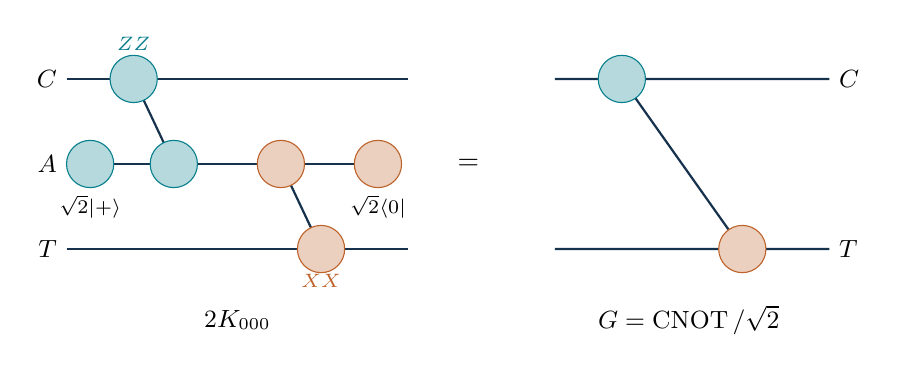
\begin{tikzpicture}[x=.85cm,y=.9cm]
\node[anchor=east,font=\small] at (0,2.4) {$C$};
\node[anchor=east,font=\small] at (0,1.2) {$A$};
\node[anchor=east,font=\small] at (0,0) {$T$};
\draw[wire] (0,2.4)--(5.1,2.4) (0,0)--(5.1,0) (.35,1.2)--(4.65,1.2);
\draw[wire] (1,2.4)--(1.6,1.2) (3.2,1.2)--(3.8,0);
\node[zs] at (1,2.4) {};\node[zs] at (1.6,1.2) {};
\node[xs] at (3.2,1.2) {};\node[xs] at (3.8,0) {};
\node[zs] at (.35,1.2) {};\node[xs] at (4.65,1.2) {};
\node[font=\scriptsize] at (.35,.6) {$\sqrt2\ket+$};
\node[font=\scriptsize] at (4.65,.6) {$\sqrt2\bra0$};
\node[font=\scriptsize,text=zc] at (1,2.9) {$ZZ$};
\node[font=\scriptsize,text=xc] at (3.8,-.45) {$XX$};
\node[font=\small] at (2.55,-1) {$2K_{000}$};
\node at (6,1.2) {$=$};
\begin{scope}[xshift=6.2cm]
\draw[wire] (0,2.4)--(1,2.4)--(4.1,2.4) (0,0)--(2.8,0)--(4.1,0) (1,2.4)--(2.8,0);
\node[zs] at (1,2.4) {};\node[xs] at (2.8,0) {};
\node[anchor=west,font=\small] at (4.1,2.4) {$C$};\node[anchor=west,font=\small] at (4.1,0) {$T$};
\node[font=\small] at (2,-1) {$G=\cnot/\sqrt2$};
\end{scope}
\end{tikzpicture}}

\begin{document}
\begin{center}
{\small\color{teal}\textbf{PART OF A SERIES OF TUTORIALS ON QUANTUM ERROR CORRECTION}}\\[9pt]
{\LARGE\bfseries\color{ink} Rotated Surface Codes}\\[10pt]
{\large From local checks to lattice surgery}\\[9pt]
{\small Revised 23 September 2026}
\end{center}
\vspace{3pt}
In the previous tutorial, we introduced stabilizers, error syndromes, and decoding, and began to examine faults in syndrome-measurement circuits. We now ask how to arrange those circuits on a device. On many platforms, including superconducting-qubit arrays, direct two-qubit gates are restricted to nearby qubits. A useful code must respect that connectivity as it grows.

We will build a surface-code patch from local checks, understand errors through its geometry, and then use joint measurements between encoded qubits to implement a logical CNOT.

\section{Locality matters}
A \textbf{geometrically local code} arranges qubits so that each check acts on a small neighborhood, even as the code grows. The surface code is one example: its checks fit on a two-dimensional lattice.

The surface code arranges data and check qubits on a two-dimensional lattice. Its short-range interactions suit hardware with local connectivity, and its geometry makes checks, error paths, and logical operators visible. Experiments also show that, under suitable conditions, logical memory errors can decrease as the code grows~\cite{google}.

\section{The rotated surface code}
The foundational constructions are Kitaev's toric code, first circulated in 1997, and Bravyi and Kitaev's planar codes with boundaries in 1998~\cite{kitaev,bravyi}; repeated noisy correction was developed further by Dennis et al.~\cite{dennis}. The conventional surface-code construction places data qubits on \textbf{edges}. An $X$ check acts on edges meeting at a vertex; a $Z$ check acts around a face. Figure~\ref{fig:layouts} uses orange and teal support shading to make these check neighborhoods explicit.

The rotated patch chooses boundaries at $45^\circ$ to the underlying lattice and trims boundary qubits. Redrawn as a square grid, its data qubits sit at the \textbf{corners of checkerboard faces}~\cite{horsman,tomita}. Both layouts are planar surface-code encodings, but their finite patches have different boundaries, check supports, and qubit counts. The rotated cut reduces the number of data qubits while preserving the intended code distance.


\begin{figure}[!ht]
\centering\layoutcomparison
\caption{Two distance-three patches. Black dots are data qubits. The dashed square highlights a conventional $Z$ face; its check acts on the four data qubits around its perimeter. In the rotated layout, each colored region acts on its data-qubit corners.}
\label{fig:layouts}
\end{figure}

% For distance $d$, the number of data qubits is: 
% \[
% n_{\mathrm{conventional}}=d^2+(d-1)^2,
% \qquad n_{\mathrm{rotated}}=d^2.
% \]
% At $d=3$, the rotated layout uses 9 rather than 13 data qubits while retaining distance three. Measurement ancillas add to both counts; fewer data qubits alone do not determine the logical error rate.

Throughout this tutorial, we draw \textcolor{xc}{$X$ checks in orange} and \textcolor{zc}{$Z$ checks in teal}. In a common implementation with one measurement ancilla per check, each colored region requires one ancilla near its center. A rotated patch then uses $d^2-1$ check ancillas in addition to its $d^2$ data qubits. Reusing ancillas can change this hardware count.

\subsection{Reading the checks and boundaries}
In the rotated patch shown here, each colored face is also called a \textbf{plaquette}. A bulk plaquette contains four data-qubit corners; a boundary half-plaquette contains two. The corresponding check multiplies the same Pauli operator over those corners:
\[
S_X(f)=\prod_{j\in\operatorname{corners}(f)}X_j,
\qquad S_Z(f)=\prod_{j\in\operatorname{corners}(f)}Z_j.
\]
In Figure~\ref{fig:patch}, the numbers run left to right along each row, beginning with 0--4 at the bottom, then 5--9 above. These labels let us name the physical operators in an example.


\begin{figure}[!ht]
\centering\detailedpatch
\caption{A distance-five patch: 25 data qubits and 24 checks. The inset highlights shared qubits 1 and 6. Boundary labels name logical operators supported \emph{along} an edge; the paths represent $\XL$ and $\ZL$, explained in the logical-operator subsection.}
\label{fig:patch}
\end{figure}

The bottom-left orange plaquette and its teal neighbor give
\[
S_X=X_0X_1X_5X_6,\qquad S_Z=Z_1Z_2Z_6Z_7.
\]
The bottom teal half-plaquette gives $Z_0Z_1$.
Every $X$--$Z$ check pair overlaps on zero or two qubits, including at boundaries. Like-type checks commute automatically. Therefore, all stabilizer checks can be imposed simultaneously. 

We assign each data vertex a \textbf{local Pauli label}\footnote{In Entropica's visual language, $\chi(q)$ may be called a
\textbf{local Pauli charge}.} by multiplying
the Pauli types of all stabilizers incident on that vertex, while
ignoring overall phase. If $n_X(q)$ and $n_Z(q)$ are the numbers of
incident $X$ and $Z$ stabilizers at vertex $q$, then
\[
\chi(q)=X^{\,n_X(q)\bmod 2}Z^{\,n_Z(q)\bmod 2}.
\]
Thus two $X$ labels cancel, two $Z$ labels cancel, and one $X$ together
with one $Z$ gives $Y$, up to phase. For example, in Figure~\ref{fig:patch},
\[
\chi(0)=XZ\sim Y,\qquad
\chi(1)=XZZ\sim X,\qquad
\chi(6)=XXZZ=I.
\]

These labels depend on the checks as drawn; they are a visual aid, not additional measured checks. They make the boundary pattern visible: along one pair
of edges their product gives $X$, and along the perpendicular pair it
gives $Z$. The stabilizer layout mathematically determines the
boundaries; the local labels provide a quick way to see them. 
In the following subsection, we use these boundary types to identify the logical
$X$ and $Z$ operators.

\subsection{Error strings, boundaries, and logical operators}\label{sec:logical}
A Pauli error changes the sign of every check with which it anticommutes. A \textbf{string} is a product of same-type Pauli errors along a path. Therefore, a check is violated exactly when it overlaps that string on an odd number of qubits. 
Thus, checks in the middle of a string usually overlap it twice and remain unchanged, while checks at its endpoints overlap it once and return $-1$. The syndrome therefore marks the string's visible endpoints.

\paragraph{One absorbed endpoint.}
Consider the bottom-left data qubit $0$. A $Z_0$ error anticommutes with the neighbouring $X$ check $X_0X_1X_5X_6$, so that check returns $-1$. The boundary check $Z_0Z_1$ commutes with $Z_0$, and there is no second $X$ check below the patch. Thus $Z_0$ has one visible endpoint and one endpoint absorbed at the bottom boundary.

In this convention, a $Z$ string creates defects on $X$ checks and may end at a top or bottom $X$ boundary. An $X$ string creates defects on $Z$ checks and may end at a left or right $Z$ boundary. At a corner the two boundary types meet. A $Y=iXZ$ error has both components; the corner is not a third, ``$Y$-boundary.''

\paragraph{Two absorbed endpoints: logical operators.}
The bottom-edge representative
\[
\XL=X_0X_1X_2X_3X_4
\]
illustrates the cancellation directly. The leftmost boundary $Z$ check
sees $X_0X_1$, the next bulk $Z$ check sees $X_1X_2$, and so on.
Every relevant $Z$ check therefore has two anticommuting overlaps and
returns $+1$. The two geometric endpoints lie on the left and right
$Z$ boundaries, where the remaining endpoint defects are absorbed.
Consequently, $\XL$ has the trivial syndrome.

However, a trivial syndrome does not imply that the logical state is
unchanged. This string connects the two distinct $Z$ boundaries of the
patch. No product of local stabilizer checks can remove such a
boundary-to-boundary path or deform it into a small region. It is
therefore not equivalent to the identity on the code space. Any $X$
string joining these two $Z$ boundaries can be deformed into this
representative by multiplying by stabilizer checks, so these strings
belong to the same logical class.

The same reasoning gives the vertical representative
\[
\ZL=Z_0Z_5Z_{10}Z_{15}Z_{20}.
\]
The edge label and the absorbing boundary should not be confused. We
draw $\XL$ \emph{along} the bottom $X$-labelled edge, but its endpoints
are absorbed at the left and right $Z$ boundaries. Similarly, $\ZL$ is
drawn along the left $Z$-labelled edge while its endpoints are absorbed
at the bottom and top $X$ boundaries.

The two representatives intersect once, at qubit $0$, so
\[
\XL\ZL=-\ZL\XL.
\]
We choose $\ZL$ as the logical $Z$ operator and define
$\ket{0_L}$ and $\ket{1_L}$ as its $+1$ and $-1$ eigenstates. The
anticommutation means that $\XL$ flips this logical $Z$ eigenvalue, so
we call it the logical $X$ operator. After fixing the relative phase
of the logical basis states,
\[
\XL\ket{0_L}=\ket{1_L},
\qquad
\XL\ket{1_L}=\ket{0_L}.
\]

\paragraph{Different boundary types and mixed errors.}
A string that reaches an incompatible boundary remains detectable. For example, a $Z$ string can begin at the bottom $X$ boundary but end at a left $Z$ boundary. The bottom endpoint is absorbed, whereas the left endpoint leaves a violated $X$ check. It has one visible $e$ defect and is not logical. The converse holds for an $X$ string from a left or right $Z$ boundary to a top or bottom $X$ boundary. 

Mixed Pauli errors should be drawn by separating their $X$ and $Z$ components. Figure~\ref{fig:error} shows $E=X_5Z_2$. The $X_5$ factor violates the $Z$ check $Z_5Z_6Z_{10}Z_{11}$, while the $Z_2$ factor violates the $X$ check $X_2X_3X_7X_8$. The error therefore produces one $m$ defect and one $e$ defect at different locations. These are not the two ends of one same-type string; they are the visible endpoints of two Pauli components.

\begin{figure}[!ht]
\centering\errorpatch
\caption{The mixed error $E=X_5Z_2$. The $X$ component violates one teal $Z$ check, producing an $m$ defect; the $Z$ component violates one orange $X$ check, producing an $e$ defect. A mixed Pauli error is drawn as its separate $X$ and $Z$ components.}
\label{fig:error}
\end{figure}

\paragraph{Zooming out with local Pauli labels.}
The local Pauli labels introduced above are useful because they make the boundary pattern visible before we draw every individual check. The square-patch picture in Figure~\ref{fig:abstract}, following the patch view in \emph{A Game of Surface Codes}~\cite{litinski}, keeps exactly the information needed here: the $X$ and $Z$ boundary types, visible syndrome defects, and the way a string connects boundaries. It hides the microscopic checks and must therefore be read using the cancellation rule established above. The local labels are a visual bookkeeping device; they are not the measured syndrome defects. The terms \emph{rough} and \emph{smooth} are also used for boundaries; with the $e/m$ convention here, rough absorbs $e$ and smooth absorbs $m$~\cite{dennis}.

\begin{figure}[!ht]
\centering\abstractstrings
\caption{Zoomed-out string classes. A $Z$ string has two visible $e$ defects in the interior, one defect after reaching a compatible $X$ boundary, or one defect after reaching an incompatible $Z$ boundary. Logical strings join distinct compatible boundaries and have no visible endpoints.}
\label{fig:abstract}
\end{figure}

\FloatBarrier

\subsection{Measuring a plaquette: gate order}

The preceding tutorial derived ancilla check measurements. An $X$ check uses an ancilla prepared in $\ket{+}$, acting as the CNOT control, and measured in $X$. A $Z$ check uses an ancilla prepared in $\ket{0}$, acting as the CNOT target, and measured in $Z$. Within an isolated, fault-free check, the order of these CNOTs does not affect the measurement. However, faults can occur during the measurement, and the order determines how they spread to the data.

For a CNOT with control $c$ and target $t$, write $U=\cnot_{c\to t}$. Pauli propagation obeys
\begin{equation}\label{eq:propagation}
\begin{aligned}
U X_c U^\dagger &= X_cX_t,
&\qquad U X_t U^\dagger &= X_t,\\
U Z_t U^\dagger &= Z_cZ_t,
&\qquad U Z_c U^\dagger &= Z_c.
\end{aligned}
\end{equation}
Thus an $X$ error spreads from control to target, while a $Z$ error spreads from target to control. In the opposite directions, these errors do not spread.

For an $X$ check, an ancilla $X$ fault can therefore propagate to several data qubits through the remaining CNOTs; an ancilla $Z$ fault does not spread to the data, although it can flip the ancilla's $X$ readout. For a $Z$ check, the roles reverse: an ancilla $Z$ fault can spread to the data, while an ancilla $X$ fault can flip the $Z$ readout. A single circuit fault that spreads through the ancilla to produce a correlated data error is called a \emph{hook error}. We therefore orient $X$-check hooks to limit their contribution to a logical $X$ error, and $Z$-check hooks to limit their contribution to a logical $Z$ error.

\begin{figure}[!ht]
\centering\schedules
\caption{CNOT orders for the patch orientation used here. Corner numbers give the time steps at which the ancilla interacts with each data qubit; they are not qubit labels. The N-shaped $X$ order makes the final pair vertical, perpendicular to a shortest logical $X$ string. The Z-shaped $Z$ order makes the final pair horizontal, perpendicular to a shortest logical $Z$ string.}
\label{fig:schedule}
\end{figure}

The key case is an ancilla fault between the second and third CNOTs\footnote{Try placing the propagating ancilla fault before, between, and after the CNOTs. Track which data qubits it reaches, then simplify the resulting error by multiplying by the measured stabilizer. A four-qubit error is the stabilizer itself, a three-qubit error is equivalent to a single-qubit error, and the two-qubit case explains the orientation choice.}: it spreads to the last two data qubits. In the N-shaped $X$ order, these form a vertical pair. Since our shortest logical $X$ strings run horizontally, this hook does not supply two neighboring sites along such a string. Similarly, the Z-shaped $Z$ order produces a horizontal pair, across rather than along a shortest vertical logical $Z$ string~\cite{tomita}. Note that these choices prevent the two-qubit hooks from providing a shortcut along the corresponding logical direction; they do not eliminate all ways a logical error can occur.

\paragraph{Can neighboring checks run together?}

Two neighboring checks share data qubits, so they cannot both interact with the same qubit at the same instant. They can nevertheless be measured during the same four-step interval: at each step, their ancillas interact with \emph{different} data qubits. This is what we mean by running the checks in parallel.

Consider the neighboring checks
\[
S_X=X_0X_1X_5X_6,
\qquad
S_Z=Z_1Z_2Z_6Z_7.
\]
They share qubits 6 and 1. Following the N-shaped and Z-shaped orders, their CNOTs are interleaved as shown below.

\begin{figure}[!ht]
\centering
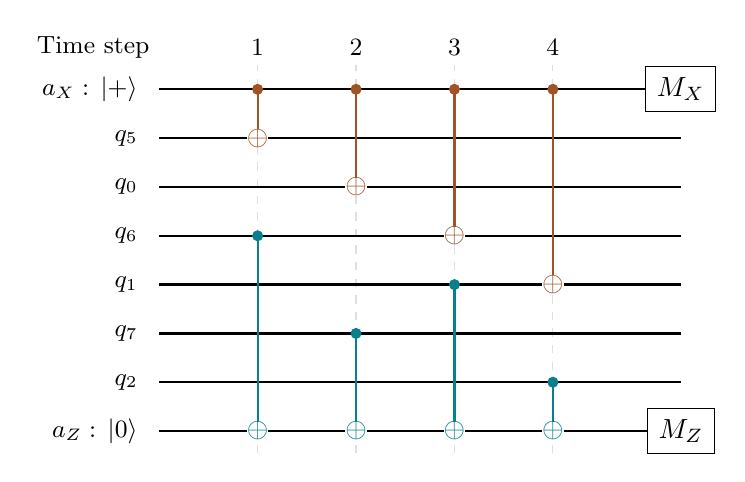
\begin{tikzpicture}[x=1.25cm,y=.62cm]
% Each column is one time step.
\foreach \x/\n in {1/1,2/2,3/3,4/4}{
  \draw[gray!25,dashed] (\x,-.45)--(\x,7.5);
  \node[font=\small] at (\x,7.85) {\n};
}
\node[anchor=east,font=\small] at (0,7.85) {Time step};

% Ancillas and data wires.
\foreach \y/\lab in {
  7/{a_X:\,|+\rangle},
  6/{q_5},
  5/{q_0},
  4/{q_6},
  3/{q_1},
  2/{q_7},
  1/{q_2},
  0/{a_Z:\,|0\rangle}
}{
  \draw[thick] (0,\y)--(5.3,\y);
  \node[anchor=east,font=\small] at (-.12,\y) {$\lab$};
}

% X-check CNOTs: ancilla controls data 5,0,6,1.
\foreach \x/\target in {1/6,2/5,3/4,4/3}{
  \draw[thick,orange!85!black] (\x,7)--(\x,\target);
  \fill[orange!85!black] (\x,7) circle (2pt);
  \node[text=orange!85!black,fill=white,inner sep=0pt]
    at (\x,\target) {$\oplus$};
}

% Z-check CNOTs: data 6,7,1,2 control the ancilla.
\foreach \x/\control in {1/4,2/2,3/3,4/1}{
  \draw[thick,teal] (\x,\control)--(\x,0);
  \fill[teal] (\x,\control) circle (2pt);
  \node[text=teal,fill=white,inner sep=0pt]
    at (\x,0) {$\oplus$};
}

% Ancilla readout.
\node[draw,fill=white,inner sep=4pt] at (5.3,7) {$M_X$};
\node[draw,fill=white,inner sep=4pt] at (5.3,0) {$M_Z$};
\end{tikzpicture}
\caption{Two neighboring check measurements in parallel.
Time runs from left to right; gates in the same numbered column
occur simultaneously. A filled dot marks a CNOT control and
$\oplus$ its target. Orange gates belong to the $X$ check and
teal gates to the $Z$ check. A vertical line crossing another
wire does not act on that wire unless a gate symbol is shown.}
\label{fig:parallel-checks}
\end{figure}

At each time step, the two ancillas interact with distinct data qubits, so there are no gate collisions. Their order must also preserve the intended parity measurements.

For example, suppose the shared qubits $q_6$ and $q_1$ start at $0,0$. In the $|1\rangle$ component of the $X$ ancilla, its CNOTs flip both bits. If the $Z$ ancilla interacts before both flips, it encounters $0,0$; after
both flips, it encounters $1,1$. Both have even parity.
But interacting before one flip and after the other gives $0,1$ or $1,0$, changing the parity.

Thus the relative order must agree at both shared qubits. Our schedule puts the $Z$ interaction first at both, so the parallel measurements preserve the intended checks.

\section{Lattice surgery: a joint logical measurement}
To compute with stored information, we need interactions between logical patches. \textbf{Lattice surgery} temporarily changes the local checks where patches meet. Their outcomes give a joint logical measurement without revealing either logical value separately~\cite{horsman}. We work through a $\ZL_L\ZL_R$ measurement, then use joint measurements to build a CNOT. The complementary Jupyter notebook explores other operations, including $\ZL_L\XL_R$.

\subsection{Measuring joint parity with local checks}
We want to measure $P=\ZL_L\ZL_R$, the logical $Z$ parity check between two distance-three patches with data qubits
$L_0,\ldots,L_8$ and $R_0,\ldots,R_8$, numbered by rows
as before. Their facing edges support
\[
\ZL_L=Z_{L_2}Z_{L_5}Z_{L_8},
\qquad
\ZL_R=Z_{R_0}Z_{R_3}Z_{R_6}.
\]
Place three additional \emph{bridge data qubits} $b_0,b_1,b_2$, each prepared in $\ket{+}$, between the patches. 
These are data qubits used to join the
patches; separate ancillas measure the new checks.

\begin{figure}[!ht]
\centering\physicalseam
\caption{An explicit $ZZ$ merge. Hollow dots are bridge data qubits, ordered bottom to top. Four highlighted $Z$ checks $G_1,\ldots,G_4$ span the seam. The other faces show the compatible checks of the merged rectangular patch. Each region is measured with a check ancilla, omitted here.}
\label{fig:seam}
\end{figure}

Measure the four new seam checks
\begin{equation}\label{eq:seam}
\begin{aligned}
G_1&=Z_{L_2}Z_{b_0},&
G_2&=Z_{b_0}Z_{b_1}Z_{R_0}Z_{R_3},\\
G_3&=Z_{L_5}Z_{L_8}Z_{b_1}Z_{b_2},&
G_4&=Z_{b_2}Z_{R_6}.
\end{aligned}
\end{equation}
In the product of the four checks, each bridge factor occurs twice and cancels because $Z_{b_i}^2=I$. Thus
\begin{equation}\label{eq:seamproduct}
G_1G_2G_3G_4=\ZL_L\ZL_R,
\qquad m=g_1\oplus g_2\oplus g_3\oplus g_4,
\end{equation}
Here $g_j=0$ denotes a $+1$ result for $G_j$, and $g_j=1$ denotes $-1$. The joint outcome bit is $m$: its measured sign is $(-1)^m$. Thus $m=0$ means the two logical $Z$ values agree, while $m=1$ means they differ.
The result $m=0$ alone does not distinguish $\ket{00}_L$ from $\ket{11}_L$.

Adding the seam $Z$ checks requires us to replace two old $X$ checks at the facing boundaries. For example, the old left check $B_L=X_{L_2}X_{L_5}$ anticommutes with $G_1$ because they overlap only at $L_2$. Suppose a seam measurement gives $G_1\ket{\psi}=\ket{\psi}$. If we then measure $B_L$ and obtain $+1$, the state is proportional to $(I+B_L)\ket{\psi}$. But
\[
G_1\ket{\psi}=\ket{\psi},
\qquad
G_1B_L\ket{\psi}=-B_L\ket{\psi}.
\]
The two terms have opposite $G_1$ signs. Measuring $G_1$ again gives either sign with equal probability, even though no data error occurred. The old check $B_L$ therefore cannot remain a check of the merged patch. The old right check $X_{R_3}X_{R_6}$ similarly conflicts with $G_2$.

We replace them with
\[
H_L=X_{L_2}X_{L_5}X_{b_0}X_{b_1},
\qquad
H_R=X_{b_1}X_{b_2}X_{R_3}X_{R_6}.
\]
Each replacement has an even number of overlaps with
every seam $Z$ check, so they commute. Both start with
sign $+1$, because they are products of an old $X$
check and $X$ operators on bridge qubits prepared in
$\ket{+}$. Together with the retained checks, they
define the merged patch.

\subsection{Splitting and accounting for the outcomes}

The merge has measured the joint parity. To separate the patches again, measure the three bridge qubits in $X$ and restore the old boundary checks. Let $r_i=0$ mean an $X_{b_i}$ result of $+1$, and $r_i=1$ mean $-1$.

Before the split, the replacement checks $H_L$ and $H_R$ have sign $+1$. Using their definitions, the restored boundary checks must therefore have signs
\[
X_{L_2}X_{L_5}:\ (-1)^{r_0\oplus r_1},
\qquad
X_{R_3}X_{R_6}:\ (-1)^{r_1\oplus r_2}.
\]
For example, if $r_0\oplus r_1=1$, the left boundary check has sign $-1$ in order to have $H_L$ $+1$. This is a known outcome of the
split, not an unknown data error.

The bridge measurements also affect the signs between terms in the data state. Consider the middle bridge qubit $b_1$.
Its $X$ measurement gives either
$\ket{+}=(\ket0+\ket1)/\sqrt2$ or $\ket{-}=(\ket0-\ket1)/\sqrt2$.
Compared with a $\ket{+}$ result, a $\ket{-}$ result puts a minus sign on the part of the state paired with $b_1=1$.

The seam checks tell us how that sign appears on the data:
\[
G_1G_2=Z_{L_2}Z_{b_1}Z_{R_0}Z_{R_3}.
\]
Once the outcomes of $G_1$ and $G_2$ are known, the extra minus signs from a $\ket{-}$ result on $b_1$ have the same effect on the data as $Z_{L_2}Z_{R_0}Z_{R_3}$, apart from an overall sign. We can write this data operator as
\[
Z_{L_2}Z_{R_0}Z_{R_3}
=Z_{L_2}Z_{R_6}\ZL_R.
\]
The first two factors affect local boundary-check signs, while the last factor is a logical $Z$ on the right logical qubit. 
Accounting for all three bridge outcomes gives
\begin{equation}\label{eq:splitframe}
D_{\mathbf r}
=Z_{L_2}^{\,r_0\oplus r_1}
 Z_{R_6}^{\,r_1\oplus r_2}
 \ZL_R^{\,r_1}.
\end{equation}
The first two factors account for the restored boundary-check signs; the last records the logical $Z$ effect. We keep track of $D_{\mathbf r}$ in a \textbf{Pauli frame}: a classical record used to interpret later measurements, without applying extra physical gates.

\begin{figure}[!ht]
\centering\surgerydiagram
\caption{Join the patches to measure their joint parity, then measure the bridge qubits to separate them. Their outcomes determine the Pauli frame in Eq.~\eqref{eq:splitframe}.}
\end{figure}

This description assumes ideal measurements. With noisy measurements, the seam checks must be repeated and decoded before their joint parity can be trusted. Exchanging $X$ and $Z$ gives a joint $XX$ measurement on facing $X$ edges. At the logical level, a $\ZL_L\XL_R$ measurement can be understood by applying a Hadamard basis change to the right patch, measuring $\ZL_L\ZL_R$, and undoing the basis change. Implementing that basis change is an additional operation, not part of the $ZZ$ seam shown here.

We now use $ZZ$ and $XX$ measurements to build a CNOT.

\section{A CNOT using an ancillary logical patch}
Let $C$ and $T$ be arbitrary control and target logical qubits. Prepare a third logical patch $A$ in $\ket{+}_L$. In this section, $X_C,Z_C$, and analogous symbols denote \emph{logical} Paulis; we omit overbars to keep the derivation readable.
The table below shows the procedure for applying a CNOT between two logical patches.
\begin{center}
\begin{tabular}{clc}
\toprule
Step & Measurement & Result bit\\
\midrule
1 & $Z_CZ_A$ & $a$\\
2 & $X_AX_T$ & $b$\\
3 & $Z_A$    & $c$\\
\bottomrule
\end{tabular}
\end{center}

For each result bit, $0$ means a measured sign of $+1$ and $1$ means $-1$. Each split updates the Pauli frame used to interpret later results. The bits $a,b,c$ denote logical outcomes interpreted using the current frame. Patch $A$ is then no longer needed for this CNOT and can be reset for later use.

The three results tell us which known Pauli correction accompanies the CNOT:
\[
F=Z_C^{\,b}X_T^{\,a\oplus c}.
\]
For example, if $a=1$ and $b=c=0$, then $F=X_T$: the target has a known extra $X$. We can correct it physically, or record $F$ in the \textbf{Pauli frame} and use that record to interpret later measurements.

\begin{figure}[!ht]
\centering\cnotpatches
\caption{An L-shaped layout: $C$ and $A$ meet on $Z$ edges; $A$ and $T$ meet on $X$ edges. The highlighted seams are used successively, with the patches split again after each parity operation. The last panel measures the ancillary logical patch.}
\end{figure}

\subsection{Checking the CNOT by tracking logical operators}

We can verify the CNOT without following every possible input state.
Instead, we track the four logical Pauli operators $X_C,Z_C,X_T,Z_T$ through the measurements.
For an ideal CNOT with control $C$ and target $T$, the expected rules are
\[
X_C\longmapsto X_CX_T,\qquad
Z_C\longmapsto Z_C,\qquad
X_T\longmapsto X_T,\qquad
Z_T\longmapsto Z_CZ_T.
\]
We will show that our measurement procedure gives these rules, apart from signs determined by its known outcomes.

Start with $X_C$. The ancilla was prepared in $\ket{+}_L$, so initially $X_A=+1$ and $X_C$ acts like $X_CX_A$. 
This operator commutes with both joint measurements: it has two anticommuting overlaps with $Z_CZ_A$ and commutes with $X_AX_T$. After the second measurement, $X_AX_T=(-1)^b$, so $X_A$ acts like $(-1)^bX_T$.
Thus $X_C$ reaches the output as
\[
X_C\longmapsto(-1)^bX_CX_T.
\]

Now consider $Z_T$. After the first measurement,
$Z_CZ_A=(-1)^a$, so $Z_T$ acts like
$(-1)^aZ_CZ_AZ_T$. This operator commutes with
$X_AX_T$: it anticommutes on both $A$ and $T$,
giving two minus signs that cancel. The final
measurement gives $Z_A=(-1)^c$. Hence
\[
Z_T\longmapsto(-1)^{a\oplus c}Z_CZ_T.
\]
The other two operators, $Z_C$ and $X_T$, commute
with all three measurements and remain unchanged.
The four rules are therefore
\[
\begin{aligned}
X_C&\longmapsto(-1)^bX_CX_T,
& Z_C&\longmapsto Z_C,\\
X_T&\longmapsto X_T,
& Z_T&\longmapsto(-1)^{a\oplus c}Z_CZ_T.
\end{aligned}
\]

A CNOT has these same rules without the two
outcome-dependent signs. These four Pauli rules determine the two-qubit operation up to an overall scalar. Both signs are accounted for by the known Pauli $F=Z_C^{\,b}X_T^{\,a\oplus c}$.
For example, $Z_C$ changes the sign of $X_C$ when
$b=1$, while $X_T$ changes the sign of $Z_T$ when
$a\oplus c=1$. Recording $F$ in the Pauli frame
therefore leaves exactly the logical action of a
CNOT, for any input state.

Each measurement has two equally likely outcomes:
$Z_CZ_A$ is unbiased because $A$ starts in
$\ket{+}_L$; $X_AX_T$ is unbiased after the first
measurement because it anticommutes with $Z_CZ_A$;
and $Z_A$ is unbiased after the second because it
anticommutes with $X_AX_T$. Each branch thus has
probability $1/8$. If $K_{abc}$ denotes its
unnormalized operation, we have
\begin{equation}\label{eq:cnotkraus}
K_{abc}\doteq
\frac{1}{2\sqrt2}\,
Z_C^{\,b}X_T^{\,a\oplus c}\cnot_{C\to T},
\end{equation}
where $\doteq$ means equality up to an overall
phase, which has no effect on the state.

We have moved from local checks to a logical CNOT: seam checks reveal joint parity, and the measurement outcomes determine the Pauli frame. This ideal operator argument does not establish fault tolerance. The next tutorial examines noisy measurements, repeated rounds, and decoding.

\begin{thebibliography}{9}
\bibitem{kitaev} A. Kitaev, \emph{Fault-tolerant quantum computation by anyons}, Ann. Phys. 303, 2--30 (2003); preprint 1997. \href{https://arxiv.org/abs/quant-ph/9707021}{arXiv:quant-ph/9707021}.
\bibitem{bravyi} S. B. Bravyi and A. Yu. Kitaev, \emph{Quantum codes on a lattice with boundary} (1998). \href{https://arxiv.org/abs/quant-ph/9811052}{arXiv:quant-ph/9811052}.
\bibitem{dennis} E. Dennis, A. Kitaev, A. Landahl, and J. Preskill, \emph{Topological quantum memory}, J. Math. Phys. 43, 4452--4505 (2002). \href{https://arxiv.org/abs/quant-ph/0110143}{arXiv:quant-ph/0110143}.
\bibitem{horsman} C. Horsman, A. G. Fowler, S. Devitt, and R. Van Meter, \emph{Surface code quantum computing by lattice surgery}, New J. Phys. 14, 123011 (2012). \href{https://arxiv.org/abs/1111.4022}{arXiv:1111.4022}.
\bibitem{litinski} D. Litinski, \emph{A Game of Surface Codes: Large-Scale Quantum Computing with Lattice Surgery}, Quantum 3, 128 (2019). \href{https://quantum-journal.org/papers/q-2019-03-05-128/}{doi:10.22331/q-2019-03-05-128}.
\bibitem{google} Google Quantum AI and Collaborators, \emph{Quantum error correction below the surface code threshold}, Nature 638, 920--926 (2025). \href{https://doi.org/10.1038/s41586-024-08449-y}{doi:10.1038/s41586-024-08449-y}.
\bibitem{tomita} Y. Tomita and K. M. Svore, \emph{Low-distance surface codes under realistic quantum noise}, Phys. Rev. A 90, 062320 (2014). \href{https://arxiv.org/abs/1404.3747}{arXiv:1404.3747}.
\end{thebibliography}
\end{document}
